%%%%%%%%%%%%%%%%%%%%%%%%%%% asme2e.tex %%%%%%%%%%%%%%%%%%%%%%%%%%%%%%%
% Template for producing ASME-format articles using LaTeX            %
% Written by   Harry H. Cheng                                        %
%              Integration Engineering Laboratory                    %
%              Department of Mechanical and Aeronautical Engineering %
%              University of California                              %
%              Davis, CA 95616                                       %
%              Tel: (530) 752-5020 (office)                          %
%                   (530) 752-1028 (lab)                             %
%              Fax: (530) 752-4158                                   %
%              Email: hhcheng@ucdavis.edu                            %
%              WWW:   http://iel.ucdavis.edu/people/cheng.html       %
%              May 7, 1994                                           %
% Modified: February 16, 2001 by Harry H. Cheng                      %
% Modified: January  01, 2003 by Geoffrey R. Shiflett                %
% Use at your own risk, send complaints to /dev/null                 %
%%%%%%%%%%%%%%%%%%%%%%%%%%%%%%%%%%%%%%%%%%%%%%%%%%%%%%%%%%%%%%%%%%%%%%%%
%%%%%%%%%%%%%%%%%%%%%%%%%%%%%%%%%%%%%%%%%%%%%%%%%%%%%%%%%%%%%%%%%%%%%%%%

%%% use twocolumn and 10pt options with the asme2e format
\documentclass[twocolumn,10pt]{asme2e}
\usepackage{graphicx}      % include this line if your document contains figures
\usepackage{multirow}
\usepackage{amsfonts}
\usepackage{amsmath}
\usepackage{mathptmx}
\usepackage[linecolor=black,backgroundcolor=lightgray]{todonotes}
\DeclareMathAlphabet{\mathcal}{OMS}{cmsy}{m}{n}
\special{papersize=8.5in,11in}

%% The class has several options
%  onecolumn/twocolumn - format for one or two columns per page
%  10pt/11pt/12pt - use 10, 11, or 12 point font
%  oneside/twoside - format for oneside/twosided printing
%  final/draft - format for final/draft copy
%  cleanfoot - take out copyright info in footer leave page number
%  cleanhead - take out the conference banner on the title page
%  titlepage/notitlepage - put in titlepage or leave out titlepage
%  
%% The default is oneside, onecolumn, 10pt, final

%%% Replace here with information related to your conference
\confshortname{IMECE 2021}
\conffullname{IMECE International Mechanical Engineering Congress \& Exposition}

%%%%% for date in a single month, use
%\confdate{24-28}
%\confmonth{September}
%%%%% for date across two months, use
\confdate{1-5}
\confmonth{November}
\confyear{2021}
\confcity{Virtual Conference, Online}
\confcountry{USA}

%%% Replace DETC2009/MESA-12345 with the number supplied to you 
%%% by ASME for your paper.
\papernum{IMECE2021-70012}

%%% You need to remove 'DRAFT: ' in the title for the final submitted version.
\title{Specifying the Spring Constant of a Monopode Jumping System with Reinforcement Learning}
%%% for the discussion section only
%\usepackage{helvet}
%\title{\fontfamily{phv}\selectfont{\Huge{DRAFT: AN ARTICLE CREATED USING \LaTeX2\raisebox{-.3ex}{$\epsilon$}\ IN ASME FORMAT}}}

%%% first author
\author{Andrew Albright
    \affiliation{
	Department of Mechanical Engineering\\
	University of Louisiana at Lafayette\\
	Lafayette, Louisiana 70504\\
    andrew.albright1@louisiana.edu
    }	
}

%%% second author
%%% remove the following entry for single author papers
%%% add more entries for additional authors
\author{Joshua Vaughan
    %    {\tensfb Second Coauthor}
    \affiliation{Department of Mechanical Engineering\\
	University of Louisiana at Lafayette\\
	Lafayette, Louisiana, 70504\\
	joshua.vaughan@louisiana.edu
    }
}

\begin{document}

\maketitle    

%%%%%%%%%%%%%%%%%%%%%%%%%%%%%%%%%%%%%%%%%%%%%%%%%%%%%%%%%%%%%%%%%%%%%%%%
%%%%%%%%%%%%%%%%%%%%%%%%%%%%%%%%%%%%%%%%%%%%%%%%%%%%%%%%%%%%%%%%%%%%%%%%
\begin{abstract}
{\it Legged systems have many advantages when compared to their wheeled counterparts. For example, they can more easily navigate extreme, uneven terrain. However, there are disadvantages as well, including difficulties seen in modeling the nonlinearities of the system. Research has shown that using flexible components is advantageous in terms of both efficiency and legged locomotive performance. Because of the difficulties encountered in modeling flexible systems, control methods such as reinforcement learning can be used to define control strategies. Furthermore, reinforcement learning can be tasked with learning mechanical parameters of a system to match a control input. It is shown in this work that by deploying reinforcement learning to solve for the optimal spring constant for a pogo-stick jumping system, designs which the agent defines are shown to be higher performing in terms of jumping height.}
\end{abstract}

%%%%%%%%%%%%%%%%%%%%%%%%%%%%%%%%%%%%%%%%%%%%%%%%%%%%%%%%%%%%%%%%%%%%%%%%
%%%%%%%%%%%%%%%%%%%%%%%%%%%%%%%%%%%%%%%%%%%%%%%%%%%%%%%%%%%%%%%%%%%%%%%%
% \begin{nomenclature}
% \entry{A}{You may include nomenclature here.}
% \entry{$\alpha$}{There are two arguments for each entry of the nomemclature environment, the symbol and the definition.}
% \end{nomenclature}

%%%%%%%%%%%%%%%%%%%%%%%%%%%%%%%%%%%%%%%%%%%%%%%%%%%%%%%%%%%%%%%%%%%%%%%%
%%%%%%%%%%%%%%%%%%%%%%%%%%%%%%%%%%%%%%%%%%%%%%%%%%%%%%%%%%%%%%%%%%%%%%%%
\section{Introduction}
\label{sec:intro}
%
The use of flexible components within legged locomotive systems has proved useful for both reducing power consumption and increasing performance \cite{Sugiyama2004, Buondonno2017, Hurst2008}. However, designing controllers for these systems is difficult as the flexibility of the system generates nonlinear models. As such, employing series-elastic-actuators (SEA) instead of flexible links is an attractive and popular solution, since the models of the systems become more manageable \cite{Buondonno2017, Zhang2019, Pratt1995}. Still, the use of SEAs do not represent the full capability of flexible systems. As a result, other methods that use flexible tendon-like materials meant to emulate more organic designs have been proposed \cite{Iida2005}. These however are still not representative of fully flexibly links which have been shown to drastically increase locomotive performance measures such as running speed \cite{Saranli2001}.

Control methods have been developed that work well for flexible systems like the ones mentioned \cite{Luo1993, Modeling2003}. However, as the systems increase in dimensionality, effects such as dynamic coupling between members make such methods challenging to implement. As such, work has been done which uses neural networks and methods such as reinforcement learning (RL) to develop controllers for flexible systems \cite{Bhagat2019e, Thuruthelb}. For example, RL has been used to create faster running control strategies for flexible-legged locomotive systems that also are robust to different design parameters \cite{Dwiel2019d}.

In addition to the work done using RL to develop controllers for flexible systems, work has been completed which shows that this technique can be used to concurrently design the mechanical aspects of a system and a controller to match said system \cite{Ha2019j}. These techniques have even been used to define mechanical parameters and control strategies where the resulting controller and hardware were deployed in a sim-to-real process, validating the usability of the technique \cite{Chen2020}. Using this technique for legged-locomotion has also been studied, but thus far has been limited to the case of rigid systems \cite{Schaff2019e}. 

As such, this paper starts the discovery of using RL for concurrent design of flexible-legged locomotive systems. A simplified flexible jumping system was used where, for the initial work, the control input was held fixed so that the RL algorithm was tasked with only learning optimized mechanical parameters. The rest of the paper is organized such that in the next section, similar work will be discussed. In Section \ref{sec:model}, the pogo-stick environment details will be defined. Then, in Sections \ref{sec:RL}, the RL algorithm and environment used in this work will be introduced. The performance of the proposed algorithm is presented in \ref{sec:results}. % Leaving conclusion section out intentionally

%%%%%%%%%%%%%%%%%%%%%%%%%%%%%%%%%%%%%%%%%%%%%%%%%%%%%%%%%%%%%%%%%%%%%%%%
%%%%%%%%%%%%%%%%%%%%%%%%%%%%%%%%%%%%%%%%%%%%%%%%%%%%%%%%%%%%%%%%%%%%%%%%
\section{Related Work}
\label{sec:related_work}

%%%%%%%%%%%%%%%%%%%%%%%%%%%%%%%%%%%%%%%%%%%%%%%%%%%%%%%%%%%%%%%%%%%%%%%%
\subsection{Flexible Locomotive Systems}
\label{sec:flexible_background}
%
The use of flexible components within robotics systems has shown improvements in performance measures specifically ones which are locomotive \cite{Hurst2008}. In particular, advantages have been seen in locomotion applications where crawling and jumping are employed \cite{Sugiyama2004}. Previous work has shown that the use of flexible components in the legs of legged locomotion systems increase performance while decreasing power consumption \cite{Saranli2001}. Related to work on robotics systems employing flexible links, work has been done showing the uses of series-elastic-actuators for locomotive systems \cite{Pratt1995}. In much of this work, human interaction with the robotic systems is considered where rigidity is not ideal \cite{Zhang2019}. The studies of flexible systems are challenging however, as the models which represent them are often nonlinear and therefore difficult to develop control systems for. As such, there is a need for solutions which can be deployed to develop controllers for these nonlinear systems.
	
%%%%%%%%%%%%%%%%%%%%%%%%%%%%%%%%%%%%%%%%%%%%%%%%%%%%%%%%%%%%%%%%%%%%%%%%	
\subsection{Controlling Flexile Systems Using RL}
\label{sec:control_rl}
%
Control methods developed for flexible linked systems have been shown to be effective for position control and vibration reduction \cite{Luo1993, Ahmadi1997}. Because of the challenges seen in scaling the controllers, methods utilizing reinforcement learning are of interest. This method has been used in simple planar cases, where it is compared to a PD control strategy for vibration suppression and proves to be a higher performing method \cite{He2020f}. Additionally, it has also been shown to be effective at defining control strategies for flexible-legged locomotion. The use of actor-critic algorithms such as Deep Deterministic Policy Gradient \cite{Lillicrap2016h} have been used to train running strategies for a flexible legged quadruped \cite{Dwiel2019d}. Much of the research is based in simulation, however, and often the controllers are not deployed in a sim-to-real fashion which leads to the question on whether or not these are practically useful techniques.

%%%%%%%%%%%%%%%%%%%%%%%%%%%%%%%%%%%%%%%%%%%%%%%%%%%%%%%%%%%%%%%%%%%%%%%%
\subsection{Concurrent Design}
\label{sec:control_design}
%
Defining an optimal controller for a system can be challenging due to things like mechanical and electrical design limits. This is especially true when the system is flexible and the model is nonlinear. A solution to this challenge is to concurrently design a system with the controllers so that the two are jointly optimized. This is has been researched in previous work as a strategy to develop better performing mechatronics systems \cite{Li2001}.  More recent work has been completed which used advanced methods such as evolutionary strategies to define robot design parameters \cite{Wang2019}. In addition to evolutionary strategies, reinforcement learning has been shown to be a viable solution for concurrent design of 2D simulated locomotive systems \cite{Ha2019j}. This is further shown to be a viable method by demonstrating more complex morphology modifications in 3D reaching and locomotive tasks \cite{Schaff2019e}. However, these techniques have not been applied to flexible systems for locomotive tasks. 



%%%%%%%%%%%%%%%%%%%%%%%%%%%%%%%%%%%%%%%%%%%%%%%%%%%%%%%%%%%%%%%%%%%%%%%%
%%%%%%%%%%%%%%%%%%%%%%%%%%%%%%%%%%%%%%%%%%%%%%%%%%%%%%%%%%%%%%%%%%%%%%%%
\section{Pogo-stick Model}
\label{sec:model}
%
	\begin{figure}[t]
		\begin{center}
			\includegraphics[width=2.5cm]{figures/pogo_system.pdf}
		\end{center}
		\caption{Pogo-stick System}
		\label{fig:pogoStickSystem} 
	\end{figure}

	\begin{table}[t]
		\caption{POGO-STICK MODEL PARAMETERS}
		\begin{center}
		\label{tab:pogoStickSystem}
			\begin{tabular}{l l}
%			& & \\ % put some space after the caption
			\textbf{Model Parameter} & \textbf{Value}\\
			\hline
			\hline
			Mass of Leg & 0.175 kg\\
			Mass of Actuator & 1.003 kg \\
			Spring Constant, $k$ & 50000--350000 $\mbox{N}/\mbox{m}$ \\
			Actuator Stroke, $(x_{a})_{\mbox{max}}$ & 25.0 $\mbox{mm}$ \\
			Max.\ Actuator Velocity, $(\dot{x}_{a})_{\mbox{max}}$ & 1.0 $\mbox{m}/\mbox{s}$ \\ 
			Max.\ Actuator Accel., $(\ddot{x}_{a})_{\mbox{max}}$ & 10.0 $\mbox{m}/\mbox{s}^2$\\
			\end{tabular}
		\end{center}
		\vspace{-0.2in}
	\end{table}

The pogo-stick model show in Figure~\ref{fig:pogoStickSystem} has been shown to be useful as a representation of several different running and jumping gaits \cite{Blickhan1993a}. As such, it is used in this work to demonstrate the ability of reinforcement learning for the initial steps of concurrent design. The models parameters are summarized in Table~\ref{tab:pogoStickSystem}. 
	
The variable $m_a$ represents the mass of the actuator, which moves along the rod with mass $m_l$. A non-linear spring with constant $k$ is used as the representation of flexibility. A damper (not shown in Figure~\ref{fig:pogoStickSystem}), is parallel to the spring. Variables $x$ and $x_a$ represent the system's vertical position with respect to the ground and the actuator's position along the rod, respectively. The system is additionally constrained such that it only moves vertically, so the reinforcement agent is not required to balance the system.
	
The equations of motion describing the system are:
%	
\begin{equation}
		\ddot{x} = \alpha \left(\frac{k}{m_t}x^3+\frac{c}{m_t}\dot{x}\right)-\frac{m_a}{m_t}\,\ddot{x}_a-g
\end{equation}
%
where $x$ and $x_a$ are position and velocity of the rod respectively, the acceleration of the actuator, $x_a$, is the control input, and $m_t$ is the mass of the complete system. Ground contact determines the value of $\alpha$, so that the spring and damper do not supply force while the leg is airborne:

	\begin{equation}
		\alpha =
		\left\{\begin{matrix}
		   -1, & x \leq 0\\ 
		   0, & \mbox{otherwise}
		   \end{matrix}\right.
	 \end{equation}


%%%%%%%%%%%%%%%%%%%%%%%%%%%%%%%%%%%%%%%%%%%%%%%%%%%%%%%%%%%%%%%%%%%%%%%%
%%%%%%%%%%%%%%%%%%%%%%%%%%%%%%%%%%%%%%%%%%%%%%%%%%%%%%%%%%%%%%%%%%%%%%%%
\section{Jumping Command Design}
\label{sec:control_input_exp}
%
Bang-bang derived jumping commands like the one shown in Figure \ref{fig:sim_command} are likely to result in a maximized jump height. For this command, the actuator mass travels at maximum acceleration within its allowable range, pauses, then accelerates in the opposite direction. Commands designed to complete this motion are bang-bang in each direction, with a selectable delay between them. The resulting motion of the actuator along the rod is shown in Figure \ref{fig:command_act_motion}. Starting from an initial position, $(x_a)_0$, it moves through a motion of stroke length $\Delta_1$, pauses there for $\delta_t$, then moves a distance $\Delta_2$ during the second portion of the acceleration input.
%
%
\begin{figure}[b]
\begin{center}
\includegraphics[width = 3in]{figures/command_form}  
\caption{Jumping Command}
\label{fig:sim_command}
\end{center}
\vspace{-0.1in}
\end{figure}
%
%
\begin{figure}[tb]
\begin{center}
\includegraphics[width = 3in]{figures/jumping_command_position}  
\caption{Resulting Actuator Motion}
\label{fig:command_act_motion}
\end{center}
%\vspace{-0.2in}
\end{figure}
%

This bang-bang-based profile can be represented as a step command convolved with a series of impulses, as shown in Figure \ref{fig:jump_convolve} \cite{Sorensen:08d}. Using this decomposition, input-shaping principles and tools can be used to design the impulse sequence \cite{Singer:90, Singhose:94a}. 
%
\begin{figure}[tbp]
\begin{center}
\includegraphics[width = 3.0in]{figures/jump_convolve}
\caption{Decomposition of the Jump Command into a Step Convolved with an Impulse Sequence}
\label{fig:jump_convolve}
\end{center}
\vspace{-0.2in}
\end{figure}
%
For the bang-bang-based jumping command, the amplitudes of the resulting impulse sequence are fixed, $A_i = [-1, 2, -1, 1, -2, 1]$. However, the impulse times, $t_i$, can be varied and optimal selection of them can lead to a maximized jump height of the pogo-stick system \cite{Vaughan2013}. Commands of this form will often result in a stutter jump like that in Figure~\ref{fig:stutterJumpFigure}, where the small initial jump allows the system to compress the spring farther storing more energy in the spring to be used in the final jump.
%
\begin{figure}[t]
	\begin{center}
		\includegraphics[width=3in]{figures/stutter_jump.pdf}
	\end{center}
	\caption{Example Stutter Jump}
	\label{fig:stutterJumpFigure} 
\end{figure}

%%%%%%%%%%%%%%%%%%%%%%%%%%%%%%%%%%%%%%%%%%%%%%%%%%%%%%%%%%%%%%%%%%%%%%%%
%%%%%%%%%%%%%%%%%%%%%%%%%%%%%%%%%%%%%%%%%%%%%%%%%%%%%%%%%%%%%%%%%%%%%%%%
\section{Learning an Optimal Spring Constant}
\label{sec:learning_spring}
%
The algorithm used for this work is Twin Delayed Deep Deterministic Policy Gradient (TD3) \cite{Fujimoto2018d}. This is an actor-critic algorithm wherein there exists two main neural networks and a set of twin trailing networks. The first main network is the actor, which determines the control input. This network takes in the systems state, $\mathcal{S}$, and outputs the action (control input), $\mathcal{A}$, based on the state. The critic is an estimator of the value of being in a state and is used to determine the difference between expected and estimated value used to update the actor network during training. It takes in the systems state, $\mathcal{S}$, and outputs the expected future reward, $\mathbb{R}$, from being in that state. The twin trailing networks are used to find the temporal difference error against the critic network which is used to update the critic network. 

To train this agent, a reinforcement learning environment conforming to the OpenAI Gym standard \cite{Brockman2016c} was created for the pogo-stick model described in Section~\ref{sec:model}, including a fixed controller input based on the algorithm described in the previous section. The agent's actions at each time step during training were selecting a spring constant. Once selected, the system was simulated, and the time series data from the simulation were used as the state transition within the RL algorithm. The reward was the maximum height that the system reached during simulation, so that the agent would learn to maximize jump height.

%%%%%%%%%%%%%%%%%%%%%%%%%%%%%%%%%%%%%%%%%%%%%%%%%%%%%%%%%%%%%%%%%%%%%%%%
%%%%%%%%%%%%%%%%%%%%%%%%%%%%%%%%%%%%%%%%%%%%%%%%%%%%%%%%%%%%%%%%%%%%%%%%
\section{Jumping Height Reached} 
\label{sec:results}
Results.

%%%%%%%%%%%%%%%%%%%%%%%%%%%%%%%%%%%%%%%%%%%%%%%%%%%%%%%%%%%%%%%%%%%%%%%%
%%%%%%%%%%%%%%%%%%%%%%%%%%%%%%%%%%%%%%%%%%%%%%%%%%%%%%%%%%%%%%%%%%%%%%%%
\section{Conclusion}
\label{sec:conclusion}
Conclusion.


%%%%%%%%%%%%%%%%%%%%%%%%%%%%%%%%%%%%%%%%%%%%%%%%%%%%%%%%%%%%%%%%%%%%%%%%
%%%%%%%%%%%%%%%%%%%%%%%%%%%%%%%%%%%%%%%%%%%%%%%%%%%%%%%%%%%%%%%%%%%%%%%%
\begin{acknowledgment}
The authors would like to thank the Louisiana Crawfish Promotion and Research Board for their support of this work.
\end{acknowledgment}

%%%%%%%%%%%%%%%%%%%%%%%%%%%%%%%%%%%%%%%%%%%%%%%%%%%%%%%%%%%%%%%%%%%%%%%%
%%%%%%%%%%%%%%%%%%%%%%%%%%%%%%%%%%%%%%%%%%%%%%%%%%%%%%%%%%%%%%%%%%%%%%%%
	
% Here's where you specify the bibliography style file.
% The full file name for the bibliography style file 
% used for an ASME paper is asmems4.bst.
\bibliographystyle{asmems4}
% Here's where you specify the bibliography database file.
% The full file name of the bibliography database for this
% article is asme2e.bib. The name for your database is up
% to you.
\bibliography{CRAWLAB-Writing-IMECE-2021}

%%%%%%%%%%%%%%%%%%%%%%%%%%%%%%%%%%%%%%%%%%%%%%%%%%%%%%%%%%%%%%%%%%%%%%%%
%%%%%%%%%%%%%%%%%%%%%%%%%%%%%%%%%%%%%%%%%%%%%%%%%%%%%%%%%%%%%%%%%%%%%%%%
% \appendix       %%% starting appendix
% \section*{Appendix A: Head of First Appendix}
% Avoid Appendices if possible.

% %%%%%%%%%%%%%%%%%%%%%%%%%%%%%%%%%%%%%%%%%%%%%%%%%%%%%%%%%%%%%%%%%%%%%%%%
%%%%%%%%%%%%%%%%%%%%%%%%%%%%%%%%%%%%%%%%%%%%%%%%%%%%%%%%%%%%%%%%%%%%%%%%
% \section*{Appendix B: Head of Second Appendix}
% \subsection*{Subsection head in appendix}
% The equation counter is not reset in an appendix and the numbers will
% follow one continual sequence from the beginning of the article to the very end as shown in the following example.
% \begin{equation}
% a = b + c.
% \end{equation}

\end{document}
